\chapter{反射与代理机制}
课前思考:
\begin{enumerate}
	\item 给定一个类的名字(字符串形式),怎么创建该类的对象?
	\item 什么是反射机制?
	\item Java静态代理和动态代理的异同有哪些?
	\item Java中的类是如何进行加载的?
\end{enumerate}
\section{Java反射机制Reflection}
\subsection{Java类型信息}
\begin{itemize}
	\item 获取Java运行时的类型信息有两种方法:
	\subitem RTTI(Run-Time Type Identification)
	\subitem Java反射机制
\end{itemize}
\subsection{RTTI}
\noindent 为什么需要RTTI?
\begin{itemize}
	\item 在运行中识别一个对象的类型;
	\item 当存储接口和其实现类时,自动转换为接口。
	\item 大部分代码尽可能少地了解对象的具体类型,而是只与对象家族中的一个通用表示打交道。
\end{itemize}
\subsection{Java反射机制的定义}
\begin{itemize}
	\item Java反射机制指的是在运行状态中,对于任意一个类,都能够知道这个类的所有属性和方法;
	对于任意一个对象,都能够调用它的任一方法和属性;这种动态获取信息以及动态调用对象方法的功能称为Java语言的反射机制。
\end{itemize}
\subsection{类Class}
Class类是Java一个基础类,每装载 一个新类的时候,JVM就会在Java堆中,创建一个Class的
实例,这个实例就代表这个Class类型,通过实例获取类型信息。该类中的一些方法如下:
\begin{itemize}
	\item Method[] getMethods()
	\item Field[] getFields()
	\item Constructor<?>[] getDeclaredContructors()
\end{itemize}
Object类中的方法:
\begin{itemize}
	\item hashCode()
	\item equals()
	\item clone()
	\item toString()
	\item notify()
	\item wait()
\end{itemize}
\subsection{利用Class类创建实例}
\begin{itemize}
	\item 创建Class的一个对象,返回一个类的引用
	\subitem
	Class cls = Class.forName("Airplane");//返回一个类型
	\item 通过类的引用创建实例
	\subitem
	cls.newInstace();
	//通过newInstace创建实例,一般调用默认构造函数
\end{itemize}
\begin{lstlisting}[language=java]
class Airplane {
	public String toString() {
		return "in airplane";
	}
}

class CreateInstance {
	public static void main(String[] args) throws ClassNotFoundException, IllegalAccessException, InstantiationException {
		Class c1 = null;
		Object ap;
		c1 = Class.forName("Airplane");
		System.out.println(c1);
		ap = c1.newInstance();
		System.out.println(ap.toString());
	}
}
//output
class Airplane
in airplane
\end{lstlisting}
\subsection{Java反射例子--Method类的invoke}
\begin{lstlisting}[language=java]
public class ClassA {
	public void add(Integer p1, Integer p2){
		System.out.println(p1.intValue() + p2.intValue());
	}
	public void StringAdd(String abc) {
		System.out.println("out" + abc);
	}
	
	public static void main(String[] args) {
		try {
			Method mth = ClassA.class.getMethod("add",new Class[]{Integer.class,Integer.class});
			mth.invoke(ClassA.class.newInstance(),new Integer(1),new Integer(2));
			Method mth1 = ClassA.class.getMethod("StringAdd",new Class[]{String.class});
			mth1.invoke(ClassA.class.newInstance(),"--test");
		} catch (Exception ex){}
	}
}
\end{lstlisting}

\section{Java静态代理}
\subsection{代理模式}
\begin{itemize}
	\item 在某些情况下,一个客户不想或者不能直接引用另一个对象,而代理对象可以在客户端
	和目标对象之间起到中介的作用。
	\item 代理模式作用:为其他对象提供一种代理以控制对这个对象的访问。
\end{itemize}
\subsection{代理模式一般涉及到的角色}
\begin{itemize}
	\item 抽象角色:声明真实对象和代理对象的共同接口。
	\item 代理角色:代理对象角色内部含有对真实对象的引用,从而操作真实对象,同时代理对象那与
	真是对象相同的接口以便在任何时刻都能够代替真实对象。同时,代理对象可以在执行真实对象操作时,附加
	其他的操作,相当于对真实对象进行封装。
	\item 真实角色:代理角色所代表的真实对象,是我们最终要引用的对象。
\end{itemize}
\subsection{静态代理例子}
\begin{lstlisting}[language=java]
//真实对象和代理对象的共同接口
public abstract class Subject {
	public abstract void request();
}
//真实角色
public class RealSubject extends Subject {
	@Override
	public void request() {
		System.out.println("From Real Subject");
	}
}
//客户端
public class Client {
	public static void main(String[] args) {
		Subject subject = new RealSubject();
		subject.request();
	}
}
//代理对象
public class ProxySubject extends Subject {
	
	private RealSubject realSubject;
	
	@Override
	public void request() {
		preRequest();
		if (realSubject == null) {
			realSubject = new RealSubject();
		}
		realSubject.request();
		postRequest();
	}
	private void preRequest(){
		System.out.println("Pre Request");
	}
	private void postRequest(){
		System.out.println("Post Request");
	}
}
\end{lstlisting}
\subsection{静态代理的优缺点}
\subsubsection{优点}
业务类只需要关注业务逻辑本身,保证了业务类的重用性,这是代理模式共有优点。
\subsubsection{缺点}
代理对象的一个接口只服务于一种类型的对象,如果要代理的方法很多,势必要为每一种方法
都进行代理,静态代理在程序规模稍大时就无法胜任了。
\par 如果接口增加一个方法,除了所有实现类需要实现这个方法外,所有代理类也需要实现此方法,增加了代码维护的复杂度。

\section{Java动态代理}
\begin{itemize}
	\item java.lang.reflect.Proxy
	\subitem 这是Java动态代理机制的主类,它提供了一组动态地生成代理类及其对象。
	\begin{lstlisting}[language=java]
//用于获取指定代理对象所关联的调用处理器
public static InvocationHandler getInvocationHandler(Object proxy)
//用于获取关联于指定类装载器和一组接口的动态代理类的类对象
public static Class<?> getProxyClass(ClassLoader loader,Class<?>... interfaces)
//用于判断指定类对象是否是一个动态代理类
public static boolean isProxyClass(Class<?> cl)
//用于为指定类装载器、一组接口及调用处理器生成动态代理类实例
public static Object newProxyInstance(ClassLoader loader,Class<?>[] interfaces,InvocationHandler h)
	\end{lstlisting}
	\item java.lang.reflect.InvocationHandler
	\subitem 这是调用处理器接口,它自定义了一个invoke方法,用于集中处理在动态代理对象上的方法调用,
	通常在该方法中实现对委托类的代理访问。
	\begin{lstlisting}[language=java]
public Object invoke(Object proxy, Method method, Object[] args)
/**该方法负责集中处理动态代理类上的所有方法调用。第一个参数是代理类实例,
 **第二个参数是被调用的方法对象,第三个参数是调用参数。
 **调用处理器根据这三个参数进行预处理或分派到委托类实例上执行。
 */
	\end{lstlisting}
\end{itemize}
\subsection{Java动态代理实例}
\begin{lstlisting}[language=java]
//代理接口
public interface Subject {
	public void request();
}
\end{lstlisting}
\begin{lstlisting}[language=java]
//真实角色
public class RealSubject implements Subject {
	public RealSubject(){}
	@Override
	public void request() {
		System.out.println("From real subject");
	}
}
\end{lstlisting}
\begin{lstlisting}[language=java]
//代理角色
public class DynamicSubject implements InvocationHandler {

	private Object sub;
	public DynamicSubject(){}
	public DynamicSubject(Object obj) {
		sub = obj;
	}

	public Object invoke(Object proxy, Method method, Object[] args) throws Throwable {
		System.out.println("before calling " + method);
		method.invoke(sub,args);
		System.out.println("after calling" + method);
		return null;
	}
}
\end{lstlisting}
\begin{lstlisting}[language=java]
//客户端调用
public class Client {
	public static void main(String[] args) {
		RealSubject rs = new RealSubject();
		InvocationHandler ds = new DynamicSubject();
		Class cls = rs.getClass();
		Subject subject = (Subject) Proxy.newProxyInstance(cls.getClassLoader(),cls.getInterfaces(),ds);
		subject.request();
	}
}
//output
before calling public abstract void Dynamic.Subject.request()
From real subject
after calling public abstract void Dynamic.Subject.request()
\end{lstlisting}
\subsection{动态代理的特点}
\begin{enumerate}
	\item 包:如果所代理的接口都是public,那么它将被定义在顶层包,
	如果所代理的接口非public,那么它将被定义在该接口所在包,这样设计目的:
	为了最大程度的保证动态代理类不会因为包管理的问题而无法被成功定义并访问。
	\item 类修饰符:该代理类具有final和public修饰符,意味着它可以被所有的类访问,
	但是不能被再度继承;
	\item 类名:格式是"\$ProxyN",其中N是一个逐一递增的数字,代表Proxy类第N次生成动态代理类,
	并不是每次调用Proxy的静态方法创建动态代理类都会使得N值增加,原因是如果对同一组接口试图重复创建动态代理类,
	它会很聪明返回先前创建好的代理类的类对象,而不会再尝试创建一个全新的代理类,可以节省不必要的代码重复生成,提高了代理类的创建效率。
	\item 类继承关系:
	\subitem 见下图
	\begin{figure}[!h]
		\centering
		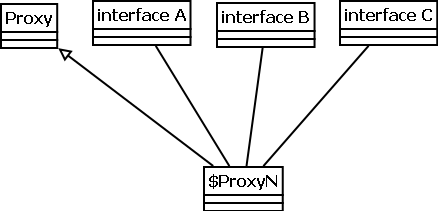
\includegraphics[width=0.6\textwidth]{image/dynamic.png}
		\caption{动态代理类继承关系}
	\end{figure}
\end{enumerate}
\subsection{动态代理优缺点}
\subsubsection{优点}
动态代理与静态代理相比较,最大优点:接口中声明的所有方法都被转移到调用处理器一个集中的方法中处理
(InvocationHandler.invoke)。这样,在接口中方法数量比较多的时候,可以灵活处理,而不需要像静态代理
那样每一个方法进行中转。
\subsubsection{缺点}
始终无法摆脱仅支持interface代理的桎梏。

\section{Java反射扩展-jvm加载类原理}
\subsection{JVM类加载的种类}
\noindent \textbf{JVM自带的默认类加载器}
\begin{enumerate}
	\item 根类加载器:bootstrap,有C++编写,所有Java程序无法获得。
	\item 扩展类加载器:由Java编写。
	\item 系统类、应用类加载器:由Java编写。
\end{enumerate}
\textbf{用户自定义的类加载器}
\par java.lang.ClassLoader的子类,用户可以定制类的加载方式。
每个类都包含了加载它的ClassLoader的一个引用-getClassLoader()。
\par 如果返回为null,证明加载它的ClassLoader是根加载器bootstrap。
\subsection{类的加载方式}
\begin{itemize}
	\item 本地编译好的class中直接加载;
	\item 网络加载:java.net.URLClassLoader可以加载url指定的类;
	\item 从jar、zip等压缩文件加载类,自动解析jar文件找到class文件去加载;
	\item 从Java源代码文件动态编译成class文件。
\end{itemize}
\subsection{类加载的步骤}
\begin{enumerate}
	\item 加载;
	\item 连接:验证、准备、解析;
	\item 类的初始化;
\end{enumerate}
\subsection{ClassLoader的加载顺序}
\noindent 加载顺序:
\par 根加载器 -> 扩展类加载器 -> 应用类加载器 -> 用户自定义类加载器
\par 如果到最后一层再加载不了就出现ClassNotFoundException异常。
\subsection{ClassLoader加载Class的过程}
\begin{enumerate}
	\item 检测此Class是否加载过,如果有直接到第8步,如果没有下一步;
	\item 如果parent classloader不存在(没有parent,那parent一定是bootstrap classloader了),
	则调到第4步;
	\item 请求parent classloader载入,如果成功到第8步,如果不成功第5步;
	\item 请求JVM从bootstrap classloader载入,如果成功第8步;
	\item 寻找Class文件(从与此classloader相关的类路径中寻找)。如果找不到则到第7步;
	\item 从文件中载入Class,到第8步;
	\item 抛出ClassNotFoundException;
	\item 返回Class。
\end{enumerate}

\section{Java进阶课程总结}
\subsection{Java线程}
\begin{itemize}
	\item 目的:多程序段执行;
	\item 安全性、互斥与同步;
\end{itemize}
\subsection{Java的网络编程}
\begin{itemize}
	\item java.net、socket通信;
\end{itemize}
\subsection{集合框架}
\begin{itemize}
	\item 集合框架关键类实现;
\end{itemize}
\subsection{JVM}
\begin{itemize}
	\item JVM、垃圾回收;
	\item Java反射机制、类加载、类代理。
\end{itemize}